\usepackage{graphicx}
\chapter{Specifikacija programske potpore}
		
	\section{Funkcionalni zahtjevi}
			
			\textbf{\textit{dio 1. revizije}}\\
			
			\textit{Navesti \textbf{dionike} koji imaju \textbf{interes u ovom sustavu} ili \textbf{su nositelji odgovornosti}. To su prije svega korisnici, ali i administratori sustava, naručitelji, razvojni tim.}\\
				
			\textit{Navesti \textbf{aktore} koji izravno \textbf{koriste} ili \textbf{komuniciraju sa sustavom}. Oni mogu imati inicijatorsku ulogu, tj. započinju određene procese u sustavu ili samo sudioničku ulogu, tj. obavljaju određeni posao. Za svakog aktora navesti funkcionalne zahtjeve koji se na njega odnose.}\\
			
			
			\noindent \textbf{Dionici:}
			
			\begin{packed_enum}
				
				\item Predsjednik neprofitabline organizacije
				\item Vlasnik kompanije
				\item Zaposlenik kompanije
					\item Kontakt
					\item Osoba zadužena za prodaju
				\item Član neprofitabline organizacije
					\item Osoba odgovorna za odnose s tvrtkama
					\item Osoba odgovorna za odnose s tvrtkama na projektu
					\item Član tima za odnose s tvrtkama
					\item Intern
				\item Administrator
				\item Razvojni tim
				
			\end{packed_enum}
			
			\noindent \textbf{Aktori i njihovi funkcionalni zahtjevi:}
			
			
			\begin{packed_enum}
				\item  \underbar{Neprijavljeni korisnik (inicijator) moze:}

				\begin{packed_enum}

					\item Ako je nadodan od strane administratora može se prijaviti svojim mailom
					\item U slučaju da je prvi neprijavljeni korisnik postaje administrator

				\end{packed_enum}

				\item  \underbar{Intern -  rola observer (inicijator) može:}
				
				\begin{packed_enum}
					
					\item Pregledavati projekte
					\item Pregledavati kompanije (naziv i područje)
					\item Pregledavati informacija o projektima (datum početka, datum završetka, oganizator)
					\item Pregledavati suradnje
					\item Pregledati korisnike
					\item Pregledati podatke o korisniku
					
				\end{packed_enum}

				\item  \underbar{Član tima za odnose s tvrtkama - rola FR team member (inicijator) može:}

				\begin{packed_enum}

					\item Pregledavati projekte
					\item Pregledavati kompanije (naziv i područje)
					\item Pregledavati informacija o projektima (datum početka, datum završetka, FR- responsiblea)
					\item Pregledavati suradnje
					\item Promijeniti podatke o suradnji (kategorija, status, sažetak, vrijednost)
					\item Pregledavati i promijeniti sve podatke za dodijeljenu kompaniju
					\item Pregledati korisnike
					\item Pregledati podatke o korisniku

				\end{packed_enum}

				\item  \underbar{Osoba odgovorna za odnose s tvrtkama na projektu -  rola FR responsible (inicijator) može:}

				\begin{packed_enum}

					\item Pregledavati projekte
					\item Pregledavati kompanije (naziv i područje)
					\item Pregledavati informacija o projektima (datum početka, datum završetka, FR- responsiblea)
					\item Pregledavati suradnje
					\item Promijeniti podatke o suradnji (kategorija, status, sažetak, vrijednost)
					\item Pregledavati i promijeniti sve podatke za dodijeljenu kompaniju
					\item Strvoriti i obrisati suradnju
					\item Pregledati korisnike
					\item Pregledati podatke o korisniku

				\end{packed_enum}

				\item  \underbar{Osoba odgovorna za odnose s tvrtkama -  rola moderator (inicijator) može:}

				\begin{packed_enum}

					\item Pregledavati projekte
					\item Pregledavati kompanije (naziv i područje)
					\item Pregledavati informacija o projektima (datum početka, datum završetka, FR- responsiblea)
					\item Pregledavati suradnje
					\item Promijeniti podatke o suradnji (kategorija, status, sažetak, vrijednost)
					\item Pregledavati i promijeniti sve podatke za dodijeljenu kompaniju
					\item Strvoriti i obrisati suradnju
					\item Stvoriti i obrisati kategoriju projekata
					\item Stvoriti i obrisati vlastito stvorene projekte
					\item Dodijeliti i maknuti nekom korisniku mogućnosti organizatora projekta na projektu koji je stvorio
					\item Staviti i maknuti nekog korisnika s rolom člana neprofitabilne kompanije na projekt koji je stvorio
					\item Pregledati korisnike
					\item Pregledati podatke o korisniku

				\end{packed_enum}

				\item  \underbar{Administrator (inicijator) može:}

				\begin{packed_enum}

					\item Pregledavati projekte
					\item Pregledavati kompanije (naziv i područje)
					\item Pregledavati informacija o projektima (datum početka, datum završetka, FR- responsiblea)
					\item Pregledavati suradnje
					\item Promijeniti podatke o suradnji (kategorija, status, sažetak, vrijednost)
					\item Pregledavati i promijeniti sve podatke za dodijeljenu kompaniju
					\item Strvoriti i obrisati suradnju
					\item Stvoriti i obrisati kategoriju projekata
					\item Stvoriti i obrisati projekte
					\item Dodijeliti nekom korisniku mogućnosti organizatora projekta na projektu koji je stvorio
					\item Staviti nekog korisnika s rolom člana neprofitabilne kompanije na projekt koji je stvorio
					\item Pregledati korisnike
					\item Pregledati podatke o korisniku
					\item Dodijeliti nekom korisniku bilo koju od prije navedenih pozicija
					\item Registrirati i maknuti korisnika iz sustava
					\item Registrirati sebe u sustav pri prvom pokretanju
					\item Promijeniti osobne podatake

				\end{packed_enum}
			
				\item  \underbar{Baza podataka (sudionik) može:}
				
				\begin{packed_enum}
					
					\item Pohranjuje sve podatke o projektima
					\item Pohranjuje sve podatke o kompanijama i njihovim kontaktima
					
				\end{packed_enum}

				\item  \underbar{Gmail api (sudionik) može:}

				\begin{packed_enum}

					\item Prijavljuje korisnika pomoću njegovog gmaila

				\end{packed_enum}
			\end{packed_enum}
			
			\eject 
			


			\subsection{Obrasci uporabe}
				
				\textbf{\textit{dio 1. revizije}}
				
				\subsubsection{Opis obrazaca uporabe}
					\textit{Funkcionalne zahtjeve razraditi u obliku obrazaca uporabe. Svaki obrazac je potrebno razraditi prema donjem predlošku. Ukoliko u nekom koraku može doći do odstupanja, potrebno je to odstupanje opisati i po mogućnosti ponuditi rješenje kojim bi se tijek obrasca vratio na osnovni tijek.}

					\noindent \underbar{\textbf{UC1 - Registracija prvog administratora}}
					\begin{packed_item}

						\item \textbf{Glavni sudionik:} Neprijavljeni korisnik
						\item \textbf{Cilj:} Stvoriti administratov korisnički račun za pristup aplikaciji
						\item \textbf{Sudionici:} Baza podataka, Google auth API
						\item \textbf{Preduvjet:} - 
						\item \textbf{Opis osnovnog tijeka:}

						\item[] \begin{packed_enum}

							\item Korisnik dolazi na stranicu koja ga preusmjerava na formu za registraciju prvog korisnika
							\item Korisnik ispunjava formu emailom prvog administratora
							\item Stranica preusmjerava korisnika na osnovnu stranicu

						\end{packed_enum}

						\item \textbf{Opis mogućih odstupanja:}

						\item[] \begin{packed_item}

							\item[2.a] Upis već postojećeg emaila ili upis korisničkih
							podatka u nedozvoljenom formatu
							\item[] \begin{packed_enum}

								\item Aplikacija obavještava korisnika o neuspjelom upisu
								\item Administrator mijenja potrebne podatke te uspješno završava unos ili
								odustaje od dodavanja novog korisnika

							\end{packed_enum}

						\end{packed_item}
					\end{packed_item}

					\noindent \underbar{\textbf{UC2 - Prijava u aplikaciju}}
					\begin{packed_item}
	
						\item \textbf{Glavni sudionik:} Neprijavljeni korisnik
						\item \textbf{Cilj:} Dati korisniku pristup aplikaciji
						\item \textbf{Sudionici:} Baza podataka
						\item \textbf{Preduvjet:} Registracija
						\item \textbf{Opis osnovnog tijeka:}
						
						\item[] \begin{packed_enum}
	
							\item Korisnik dolazi na stranicu za prijavu
							\item Otvara mu se prozor za prijavu s google računom
							\item Korisnik se prijavljuje google računom
							\item Korisnik dobiva pristup aplikaciji koja preusmjava na naslovnu stranicu
						\end{packed_enum}
						
						\item \textbf{Opis mogućih odstupanja:}

						\item[] \begin{packed_item}

							\item[2.a] Prijavom s ne- google računom
							\item[] \begin{packed_enum}

								\item Aplikacija obavještava korisnika o neuspjeloj prijavi
								\item Korisnik se ponovo prijavljuje s drugim računom ili odustaje od prijave

							\end{packed_enum}

							\item[2.b] Prijavom s računom koji nije u bazi
							\item[] \begin{packed_enum}

								\item Aplikacija obavještava korisnika o neuspjeloj prijavi
								\item Aplikacija obavještava korisnika na koju email adresu se treba javiti ako korisnik smatra da je to greška
								\item Korisnik se ponovo prijavljuje s drugim računom ili odustaje od prijave

							\end{packed_enum}

						\end{packed_item}
					\end{packed_item}

					\noindent \underbar{\textbf{UC3 - Registracija korisnika}}
					\begin{packed_item}

						\item \textbf{Glavni sudionik:} Administrator
						\item \textbf{Cilj:} Stvoriti korisnički račun za pristup aplikaciji
						\item \textbf{Sudionici:} Baza podataka
						\item \textbf{Preduvjet:} - 
						\item \textbf{Opis osnovnog tijeka:}

						\item[] \begin{packed_enum}

							\item Korisnik (administrator) odabire opciju "Users"
							\item Aplikacija prikazuje popis korisnika
							\item Korisnik odabire opciju za dodavanje korisnika
							\item Aplikacija prikaže formu za dodavanje korisnika
							\item Korisnik popuni potrebne podatke (ime, prezime, email i razinu ovlasti)
							\item Korisnik odabere opciju "Add"
							\item Baza podataka se ažurira
							\item Aplikacija zatvori formu za dodavanje korisnika
							\item Aplikacija ažurira popis korisnika
						\end{packed_enum}

						\item \textbf{Opis mogućih odstupanja:}

						\item[] \begin{packed_item}

							\item[3.a] Upis već postojećeg emaila ili upis korisničkih
							podatka u nedozvoljenom formatu
							\item[] \begin{packed_enum}

								\item Aplikacija obavještava korisnika o neuspjelom upisu
								\item Administrator mijenja potrebne podatke te uspješno završava unos ili
								odustaje od dodavanja novog korisnika

							\end{packed_enum}

						\end{packed_item}
					\end{packed_item}

					\noindent \underbar{\textbf{UC4 - Pregled projekata}}
					\begin{packed_item}

						\item \textbf{Glavni sudionik:} Intern
						\item \textbf{Cilj:} Pregledati projekte
						\item \textbf{Sudionici:} Baza podataka
						\item \textbf{Preduvjet:} Korisnik je prijavljen
						\item \textbf{Opis osnovnog tijeka:}

						\item[] \begin{packed_enum}

							\item Korisnik odabire opciju "Projects"
							\item Aplikacija prikazuje popis naziva projekata
						\end{packed_enum}
					\end{packed_item}

					\noindent \underbar{\textbf{UC5 - Pregled kompanija}}
					\begin{packed_item}

						\item \textbf{Glavni sudionik:} Intern
						\item \textbf{Cilj:} Pregledati kompanije
						\item \textbf{Sudionici:} Baza podataka
						\item \textbf{Preduvjet:} Korisnik je prijavljen
						\item \textbf{Opis osnovnog tijeka:}

						\item[] \begin{packed_enum}

							\item Korisnik odabire opciju "Companies"
							\item Aplikacija prikazuje popis kompanijama s osnovnim podacima (naziv, područje, ABC kategorizacija i link na web)
						\end{packed_enum}
					\end{packed_item}

					\noindent \underbar{\textbf{UC6 - Pregled podataka o projektu}}
					\begin{packed_item}

						\item \textbf{Glavni sudionik:} Intern
						\item \textbf{Cilj:} Pregledati podatke o projektu
						\item \textbf{Sudionici:} Baza podataka
						\item \textbf{Preduvjet:} Korisnik je prijavljen
						\item \textbf{Opis osnovnog tijeka:}

						\item[] \begin{packed_enum}

							\item Korisnik odabire opciju "Projects"
							\item Aplikacija prikazuje popis naziva projekata
							\item Korisnik klikne na naziv projekta o kojem želi informacije
							\item Prikažu se detalji projekta
						\end{packed_enum}
					\end{packed_item}

					\noindent \underbar{\textbf{UC7 - Pregled podataka o korisniku}}
					\begin{packed_item}

						\item \textbf{Glavni sudionik:} Intern
						\item \textbf{Cilj:} Pregledati podatke o željenom korisniku
						\item \textbf{Sudionici:} Baza podataka
						\item \textbf{Preduvjet:} Korisnik je prijavljen
						\item \textbf{Opis osnovnog tijeka:}

						\item[] \begin{packed_enum}

							\item Korisnik odabire opciju "Users"
							\item Aplikacija prikazuje popis korisnika
							\item Korisnik odabire željenog korisnika iz popisa
							\item Aplikacija prikazuje podatke o korisniku
						\end{packed_enum}
					\end{packed_item}

					\noindent \underbar{\textbf{UC8 - Promjena podataka o korisniku}}
					\begin{packed_item}

						\item \textbf{Glavni sudionik:} Administrator
						\item \textbf{Cilj:} Promijeniti podatke o korisniku
						\item \textbf{Sudionici:} Baza podataka
						\item \textbf{Preduvjet:} Korisnik je prijavljen, Korisnik ima razinu ovlasti administrator
						\item \textbf{Opis osnovnog tijeka:}

						\item[] \begin{packed_enum}

							\item Korisnik odabire opciju "Users"
							\item Aplikacija prikazuje popis korisnika
							\item Korisnik odabire opciju "Edit"
							\item Aplikacija prikaže formu za izmjenu podataka korisnika
							\item Korisnik mijenja podatke
							\item Korisnik odabire opciju spremi
							\item Baza podataka se ažurira
							\item Aplikacija zatvori formu za dodavanje korisnika
							\item Aplikacija ažurira popis korisnika
						\end{packed_enum}

						\item \textbf{Opis mogućih odstupanja:}

						\item[] \begin{packed_item}

							\item[2.f] Upis već postojećeg emaila ili upis korisničkih
							podatka u nedozvoljenom formatu
							\item[] \begin{packed_enum}

								\item Aplikacija obavještava korisnika o neuspjelom upisu
								\item Administrator mijenja potrebne podatke te uspješno završava unos ili
								odustaje od izmjene podataka o korisniku

							\end{packed_enum}

						\end{packed_item}
					\end{packed_item}

					\noindent \underbar{\textbf{UC9 - Pregled suradnji}}
					\begin{packed_item}
					
						\item \textbf{Glavni sudionik:} Intern
						\item \textbf{Cilj:} Pregledati podatke o suradnji
						\item \textbf{Sudionici:} Baza podataka
						\item \textbf{Preduvjet:} Korisnik je prijavljen, Korisnik je FR team member projekta
						\item \textbf{Opis osnovnog tijeka:}

						\item[] \begin{packed_enum}

							\item Korisnik odabire opciju "Projects"
							\item Aplikacija prikazuje popis naziva projekata
							\item Korisnik klikne na ime projekta u kojem se nalazi suradnja koja ga zanima
							\item Aplikacija prikazuje popis suradnji vezanih uz taj projekt sa osnovnim podacima (naziv kompanije, odgovoru osobu, status, kategoriju, kontakt, dio komentara, akcije)
						\end{packed_enum}
	
					\end{packed_item}

					\noindent \underbar{\textbf{UC10 - Promjena podataka o suradnji}}
					\begin{packed_item}

						\item \textbf{Glavni sudionik:} Član tima za odnose s tvrtkama
						\item \textbf{Cilj:} Promijeniti podatke o suradnji
						\item \textbf{Sudionici:} Baza podataka
						\item \textbf{Preduvjet:} Korisnik je prijavljen, Korisnik je FR reponsible projekta
						\item \textbf{Opis osnovnog tijeka:}

						\item[] \begin{packed_enum}

							\item Korisnik odabire opciju "Projects"
							\item Aplikacija prikazuje popis naziva projekata
							\item Korisnik klikne na ime projekta u kojem se nalazi suradnja koja ga zanima
							\item Aplikacija prikazuje popis suradnji vezanih uz taj projekt sa osnovnim podacima (naziv kompanije, odgovoru osobu, status, kategoriju, kontakt, dio komentara, akcije)
							\item Korisnik odabire opciju "Edit"
							\item Aplikacija prikaže formu s podacima te suradnje
							\item Korisnik mijenja podatke o suradnji
							\item Korisnik odabire opciju "Save"
							\item Baza podataka se ažurira
							\item Aplikacija ažurira popis suradnji

						\end{packed_enum}
						
						\item \textbf{Opis mogućih odstupanja:}

						\item[] \begin{packed_item}

							\item[1.9.b, 2.7.b] Korisnik promijeni podatke o suradnji na nevažeće vrijednosti
							i odabere opciju "Save"
							
							\item[] \begin{packed_enum}

								\item Aplikacija obavještava korisnika o neuspjelom upisu
								\item Administrator mijenja potrebne podatke te uspješno završava unos ili
								odustaje od promjene podataka

							\end{packed_enum}

						\end{packed_item}
						
					\end{packed_item}

					\noindent \underbar{\textbf{UC11 - Pregled podataka o kompaniji}}
					\begin{packed_item}

						\item \textbf{Glavni sudionik:} Član tima za odnose s tvrtkama
						\item \textbf{Cilj:} Pregledati podatke o kompaniji
						\item \textbf{Sudionici:} Baza podataka
						\item \textbf{Preduvjet:} Korisnik je prijavljen, Korisnik ima razinu ovlasti FR responsible
						\item \textbf{Opis osnovnog tijeka:}

						\item[] \begin{packed_enum}

							\item Korisnik odabire opciju "Companies"
							\item Aplikacija prikaže popis kompanija
							\item Korisnik odabire kompaniju
							\item Aplikacija prikaže detalje o toj kompaniji
						\end{packed_enum}
					\end{packed_item}

					\noindent \underbar{\textbf{UC12 - Promjena podataka o kompaniji}}
					\begin{packed_item}

						\item \textbf{Glavni sudionik:} Član tima za odnose s tvrtkama
						\item \textbf{Cilj:} Promijeniti podatke o kompaniji
						\item \textbf{Sudionici:} Baza podataka
						\item \textbf{Preduvjet:} Korisnik je prijavljen, Korisnik je odgovoran za suradnju s kompanijom
						\item \textbf{Opis osnovnog tijeka:}

						\item[] \begin{packed_enum}

							\item Korisnik odabire opciju "Companies"
							\item Aplikacija prikaže popis kompanija
							\item Korisnik odabire kompaniju za koju je dodijeljen
							\item Aplikacija prikaže podatke o kompaniji
							\item Korisnik odabire opciju "Edit"
							\item Aplikacija prikaže formu s podacima o kompaniji
							\item Korisnik mijenja podatke o kompaniji
							\item Korisnik sprema promjene
							\item Baza podataka se ažurira
							\item Aplikacija zatvori formu s podacima o kompaniji
							\item Aplikacija ažurira podatke o kompaniji
						\end{packed_enum}

						\item \textbf{Opis mogućih odstupanja:}

						\item[] \begin{packed_item}

							\item[5.b] Korisnik promijeni podatke o kompaniji na nevaljane podatke i odabere opciju "Save"
							\item[] \begin{packed_enum}

								\item Aplikacija obavještava korisnika o neuspjelom upisu
								\item Korisnik mijenja potrebne podatke te uspješno završava unos ili
								odustaje od promjene podataka

							\end{packed_enum}

						\end{packed_item}
					\end{packed_item}

					\noindent \underbar{\textbf{UC13 - Stvaranje suradnje za dodijeljen projekt}}
					\begin{packed_item}

						\item \textbf{Glavni sudionik:} Osoba odgovorna za odnose s tvrtkama na projektu
						\item \textbf{Cilj:} Stvoriti suradnju za dodijeljen projekt
						\item \textbf{Sudionici:} Baza podataka
						\item \textbf{Preduvjet:} Korisnik je prijavljen
						\item \textbf{Opis osnovnog tijeka:}

						\item[] \begin{packed_enum}

							\item Korisnik odabire opciju "Projects"
							\item Aplikacija prikazuje popis naziva projekata
							\item Korisnik klikne na ime projekta u kojem se nalazi suradnja koja ga zanima
							\item Aplikacija prikazuje popis suradnji vezanih uz taj projekt sa osnovnim podacima (naziv kompanije, odgovoru osobu, status, kategoriju, kontakt, dio komentara, akcije)
							\item Korisnik odabere opciju "New collaboration"
							\item Aplikacija prikaže formu za stvaranje nove suradnje
							\item Korisnik popunjava podatke o suradnji
							\item Korisnik sprema promjene
							\item Baza podataka se ažurira
							\item Aplikacija zatvara formu za stvaranje nove suradnje
							\item Aplikacija ažurira popis suradnji
						\end{packed_enum}

						\item \textbf{Opis mogućih odstupanja:}

						\item[] \begin{packed_item}

							\item[8.c] Korisnik unese nevaljane podatke o suradnji i odabere opciju "Save"
							\item[] \begin{packed_enum}

								\item Aplikacija obavještava korisnika o neuspjelom upisu
								\item Korisnik mijenja potrebne podatke te uspješno završava unos ili
								odustaje od dodavanja suradnje

							\end{packed_enum}

						\end{packed_item}
					\end{packed_item}

					\noindent \underbar{\textbf{UC14 - Brisanje suradnje}}
					\begin{packed_item}

						\item \textbf{Glavni sudionik:} Osoba odgovorna za odnose s tvrtkama na projektu
						\item \textbf{Cilj:} Maknuti suradnju sa dodijeljenog projekta
						\item \textbf{Sudionici:} Baza podataka
						\item \textbf{Preduvjet:} Korisnik je prijavljen
						\item \textbf{Opis osnovnog tijeka:}

						\item[] \begin{packed_enum}

							\item Korisnik odabire opciju "Projects"
							\item Korisnik klikne na ime projekta u kojem se nalazi suradnja koja ga zanima
							\item Aplikacija prikazuje popis suradnji vezanih uz taj projekt sa osnovnim podacima (naziv kompanije, odgovoru osobu, status, kategoriju, kontakt, dio komentara, akcije)
                            \item Korisnik odabere opciju za brisanje suradnje
                            \item Aplikacija pita korisnika je li siguran želi li izbrisati suradnju
                            \item Korisnik odabire potvrdnu opciju
                            \item Baza podataka se ažurira
                            \item Aplikacija ažurira popis suradnji
                            
						\end{packed_enum}
					\end{packed_item}

					\noindent \underbar{\textbf{UC15 - Stvaranje projekta}}
					\begin{packed_item}

						\item \textbf{Glavni sudionik:} Osoba odgovorna za odnose s tvrtkama
						\item \textbf{Cilj:} Stvoriti projekt
						\item \textbf{Sudionici:} Baza podataka
						\item \textbf{Preduvjet:} Korisnik je prijavljen, Korisnik ima ovlasti moderator
						\item \textbf{Opis osnovnog tijeka:}

						\item[] \begin{packed_enum}

							\item Korisnik odabire opciju "Create project"
							\item Aplikacija prikazuje formu za stvaranje novog projekta
							\item Korisnik popuni podatke za stvaranje novog projekta
							\item Korisnik sprema promjene
							\item Baza podataka se ažurira
							\item Aplikacija ažurira popis projekata
						\end{packed_enum}

						\item \textbf{Opis mogućih odstupanja:}

						\item[] \begin{packed_item}

							\item[7.b] Korisnik unese nevaljane podatke o projektu i odabere opciju "Save"
							\item[] \begin{packed_enum}

								\item Aplikacija obavještava korisnika o neuspjelom upisu
								\item Korisnik mijenja potrebne podatke te uspješno završava unos ili
								odustaje od dodavanja suradnje

							\end{packed_enum}

						\end{packed_item}
					\end{packed_item}

					\noindent \underbar{\textbf{UC16 - Brisanje projekta}}
					\begin{packed_item}
					
						\item \textbf{Glavni sudionik:} Osoba odgovorna za odnose s tvrtkama
						\item \textbf{Cilj:} Izbrisati projekt
						\item \textbf{Sudionici:} Baza podataka
						\item \textbf{Preduvjet:} Korisnik je prijavljen, Korisnik ima ovlasti administrator
						\item \textbf{Opis osnovnog tijeka:}
					
						\item[] \begin{packed_enum}

							\item Korisnik odabire opciju "Projects"
							\item Korisnik odabire neki od projekata
							\item Aplikacija prikazuje detalje o tom projektu
							\item Korisnik odabire opciju za brisanje projekta
							\item Aplikacija prikaže modal koji pita korisnika je li siguran
							\item Korisnik odabere opciju da je siguran
							\item Baza podataka se ažurira
							\item Aplikacija ažurira popis projekata
						\end{packed_enum}
					
					\end{packed_item}

						\noindent \underbar{\textbf{UC17 - Dodavanje korisnika na projekt}}
					\begin{packed_item}

						\item \textbf{Glavni sudionik:} Osoba odgovorna za odnose s tvrtkama
						\item \textbf{Cilj:} Dodati člana neprofitabilne organizacije na projekt
						\item \textbf{Sudionici:} Baza podataka
						\item \textbf{Preduvjet:} Korisnik je prijavljen, Korisnik ima ovlasti administrator
						\item \textbf{Opis osnovnog tijeka:}
					
						\item[] \begin{packed_enum}
					
							\item Korisnik odabire opciju "Projects"
							\item Aplikacija prikazuje popis projekata
							\item Korisnik odabire neki od projekata
							\item Aplikacija prikazuje detalje o tom projektu
							\item Korisnik odabire opciju za dodavanje korisnika na projekt
							\item Aplikacija prikaže formu
							\item Korisnik upiše ime, prezime, nadimak ili email člana kojeg želi dodati
							\item Korisnik odabire opciju "Add"
							\item Baza podataka se ažurira
							\item Aplikacija ažurira popis korisnika na projektu
						\end{packed_enum}
					
						\item \textbf{Opis mogućih odstupanja:}
					
						\item[] \begin{packed_item}
                        
                        	\item[7.b] Korisnik unese nevaljane podatke o korisniku i odabere opciju "Save"
							\item[] \begin{packed_enum}

								\item Aplikacija obavještava korisnika o neuspjelom upisu
								\item Korisnik mijenja potrebne podatke te uspješno završava unos ili
								odustaje od dodavanja suradnje

							\end{packed_enum}
					
						\end{packed_item}
					\end{packed_item}

					\noindent \underbar{\textbf{UC18 - Micanje korisnika sa projekta}}
					\begin{packed_item}

						\item \textbf{Glavni sudionik:} Osoba odgovorna za odnose s tvrtkama
						\item \textbf{Cilj:} Maknuti člana neprofitabilne organizacije sa projekt
						\item \textbf{Sudionici:} Baza podataka
						\item \textbf{Preduvjet:} Korisnik je prijavljen
						\item \textbf{Opis osnovnog tijeka:}

						\item[] \begin{packed_enum}

							\item Korisnik odabire opciju "Projects"
							\item Aplikacija prikazuje popis projekata
							\item Korisnik odabire neki od projekata
							\item Aplikacija prikazuje detalje o tom projektu
							\item Korisnik odabire opciju za micanje korisnika sa projekta
							\item Aplikacija prikaže modal koji pita korisnika je li siguran
							\item Korisnik odabere opciju da je siguran
							\item Baza podataka se ažurira
							\item Aplikacija ažurira popis korisnika na projektu
						\end{packed_enum}

					\end{packed_item}

					\noindent \underbar{\textbf{UC19 - Pregled korisnika}}
					\begin{packed_item}

						\item \textbf{Glavni sudionik:} Intern
						\item \textbf{Cilj:} Pregledati korisnike
						\item \textbf{Sudionici:} Baza podataka
						\item \textbf{Preduvjet:} Korisnik je prijavljen
						\item \textbf{Opis osnovnog tijeka:}

						\item[] \begin{packed_enum}

							\item Korisnik odabire opciju "Users"
							\item Aplikacija prikazuje popis korisnika
                            
						\end{packed_enum}
					\end{packed_item}

					\noindent \underbar{\textbf{UC20 - Promjena razine ovlasti korisnika}}
					\begin{packed_item}

						\item \textbf{Glavni sudionik:} Administrator
						\item \textbf{Cilj:} Promijeniti rolu korisnika
						\item \textbf{Sudionici:} Baza podataka
						\item \textbf{Preduvjet:} Korisnik je prijavljen
						\item \textbf{Opis osnovnog tijeka:}

						\item[] \begin{packed_enum}

							\item Korisnik odabire opciju "Users"
							\item Aplikacija prikazuje popis korisnika
							\item Korisnik odabere opciju za izmjenu podataka o korisniku
							\item Aplikacija prikaže formu za izmjenu podataka o korisniku
							\item Korisnik odabire jednu od razina ovlasti
							\item Korisnik odabire opciju spremi
							\item Baza podataka se ažurira
							\item Aplikacija ažurira popis korisnika

						\end{packed_enum}

						\item \textbf{Opis mogućih odstupanja:}

						\item[] \begin{packed_item}

							\item[3.a] Korisnik kojem se mijenja rola je administrator i ne postoji nijedan
							drugi administrator
							\item[] \begin{packed_enum}

								\item Sustav obavještava korisnika da mora postojati
								barem jedan administrator, pa je ova akcija zabranjena

							\end{packed_enum}

						\end{packed_item}
					\end{packed_item}

					\noindent \underbar{\textbf{UC21 - Brisanje korisnika iz sustava}}
					\begin{packed_item}

						\item \textbf{Glavni sudionik:} Administrator
						\item \textbf{Cilj:} Maknuti korisnika iz sustava
						\item \textbf{Sudionici:} Baza podataka
						\item \textbf{Preduvjet:} Korisnik je prijavljen
						\item \textbf{Opis osnovnog tijeka:}

						\item[] \begin{packed_enum}

							\item Korisnik odabire opciju "Users"
							\item Aplikacija prikazuje popis korisnika
							\item Korisnik odabere opciju brisanja željenog korisnika
							\item Aplikacija pita korisnika je li siguran da želi provesti ovu akciju
							\item Korisnik odabire opciju da je siguran
							\item Baza podataka se ažurira
							\item Aplikacija ažurira popis korisnika

						\end{packed_enum}

						\item \textbf{Opis mogućih odstupanja:}

						\item[] \begin{packed_item}

							\item[3.a] Korisnik kojem se miče iz sustava je administrator i ne postoji nijedan
							drugi administrator
							\item[] \begin{packed_enum}

								\item Sustav obavještava korisnika da mora postojati
								barem jedan administrator, pa je ova akcija zabranjena

							\end{packed_enum}

						\end{packed_item}
					\end{packed_item}

					\noindent \underbar{\textbf{UC22 - Filtriranje korisnika}}
					\begin{packed_item}

						\item \textbf{Glavni sudionik:} Intern
						\item \textbf{Cilj:} Filtrirati korisnike
						\item \textbf{Sudionici:} Baza podataka
						\item \textbf{Preduvjet:} Korisnik je prijavljen
						\item \textbf{Opis osnovnog tijeka:}

						\item[] \begin{packed_enum}

							\item Korisnik odabire opciju "Users"
							\item Aplikacija prikazuje popis korisnika
							\item Korisnik upiše tekst u polje za pretragu
							\item Aplikacija ažurira popis korisnika tako da prikazuje samo korisnike koji imaju taj tekst u imenu, prezimenu, nadimku ili emailu
						\end{packed_enum}
					\end{packed_item}
					
				\subsubsection{Dijagrami obrazaca uporabe}

					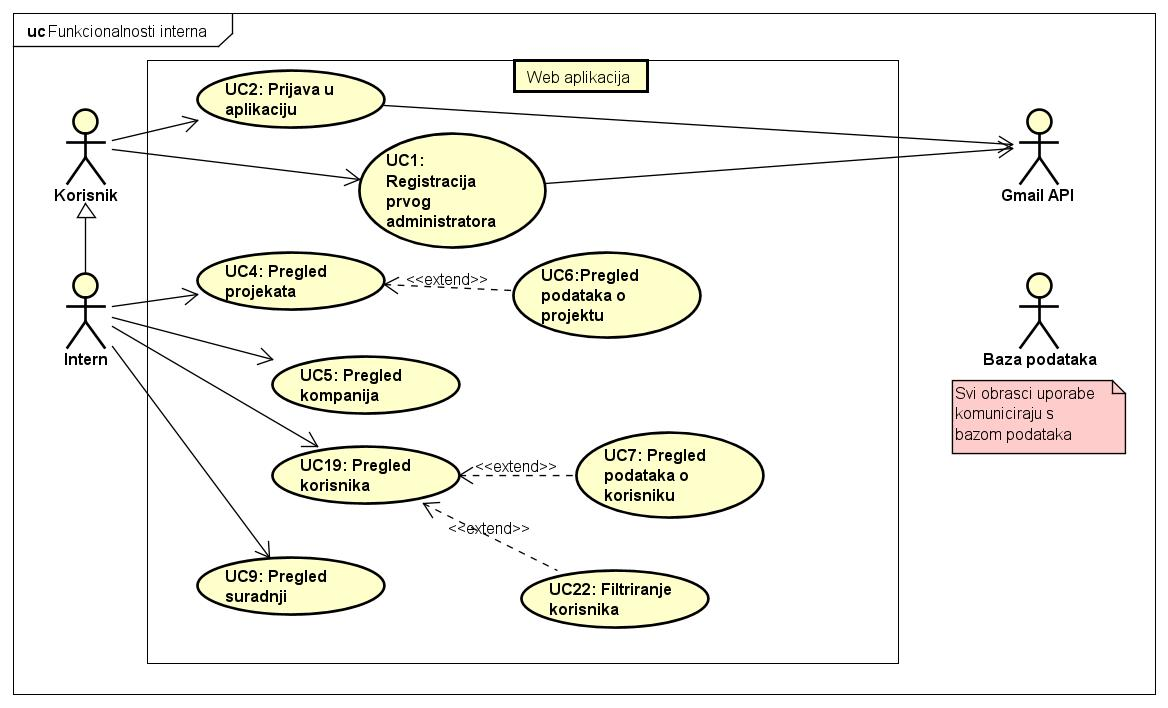
\includegraphics[width=1.25\textwidth]{./slike/UC dijagrami/UseCase observer}
					\textit{Slika 3.1: Dijagram obrasca uporabe, funkcionalnosti interna i korisnika}

					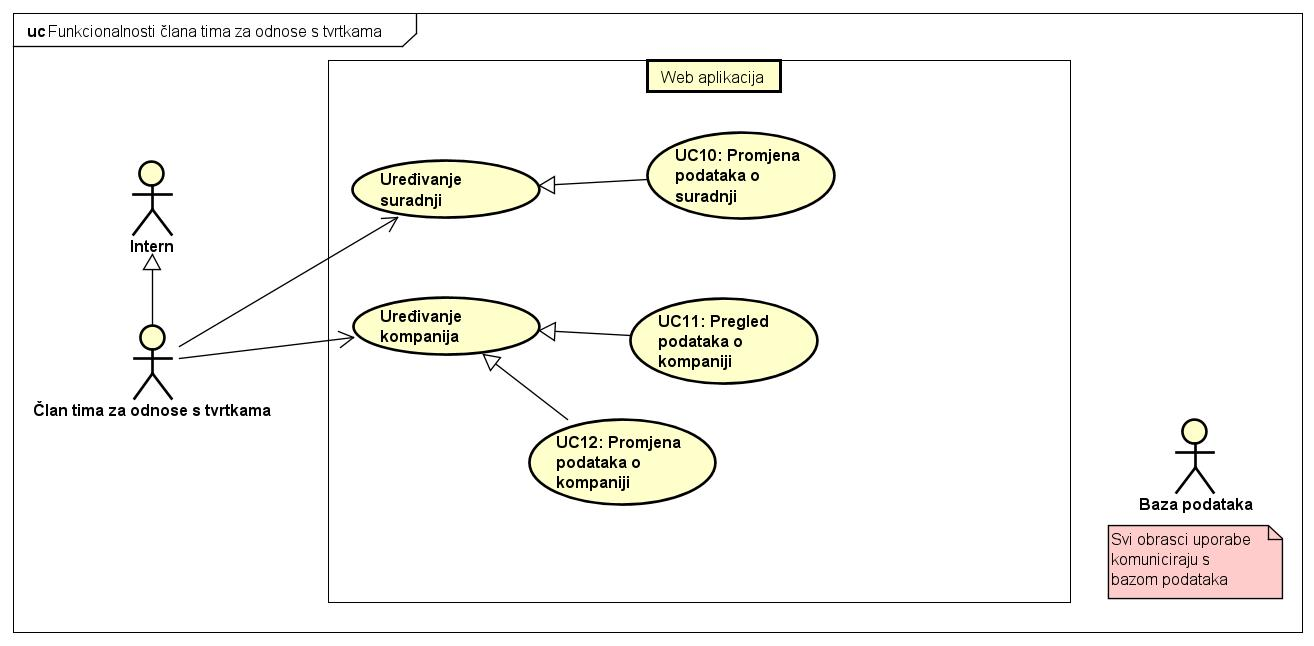
\includegraphics[width=1.25\textwidth]{./slike/UC dijagrami/UseCase FR team member}
					\textit{Slika 3.2: Dijagram obrasca uporabe, funkcionalnosti člana tima za odnose s tvrtkama}

					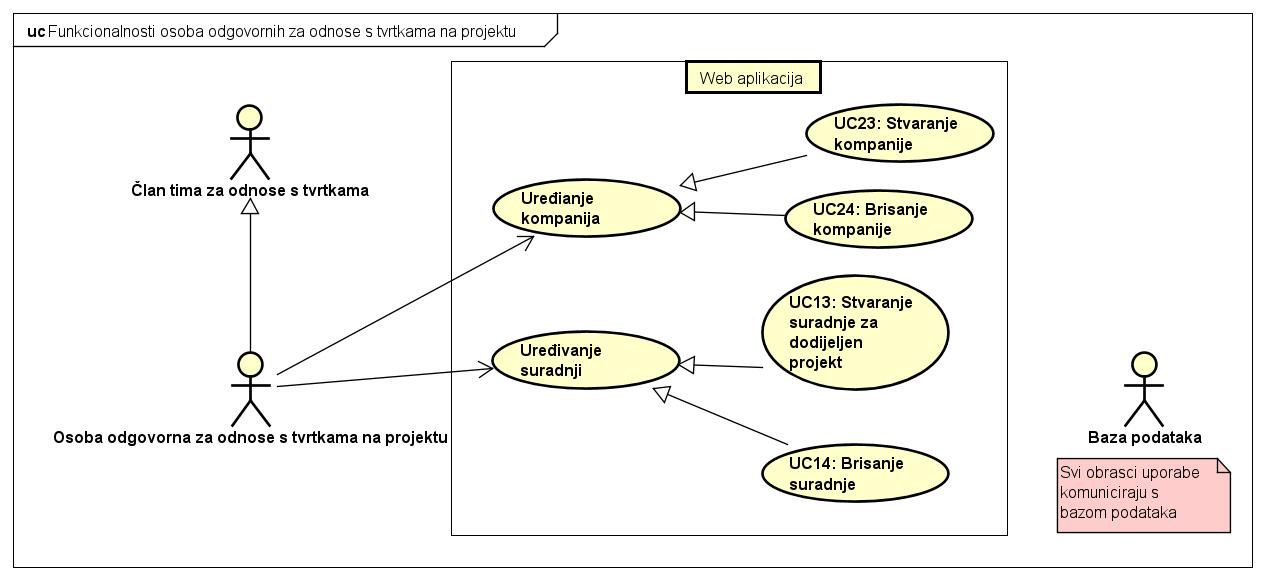
\includegraphics[width=1.25\textwidth]{./slike/UC dijagrami/UseCase FR responsible}
					\textit{Slika 3.3: Dijagram obrasca uporabe, funkcionalnosti osobe odgovorne za odnose s tvrtkama na projektu}

					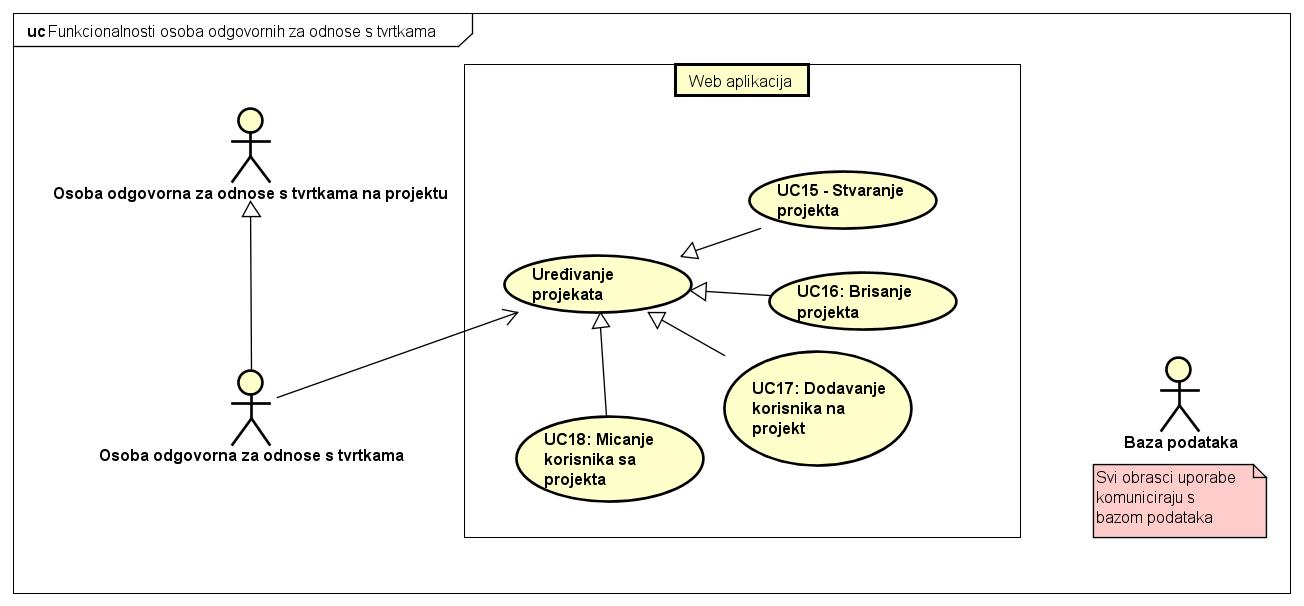
\includegraphics[width=1.25\textwidth]{./slike/UC dijagrami/UseCase moderator}
					\textit{Slika 3.4: Dijagram obrasca uporabe, funkcionalnosti osobe odgovorne za odnose s tvrtkama}

					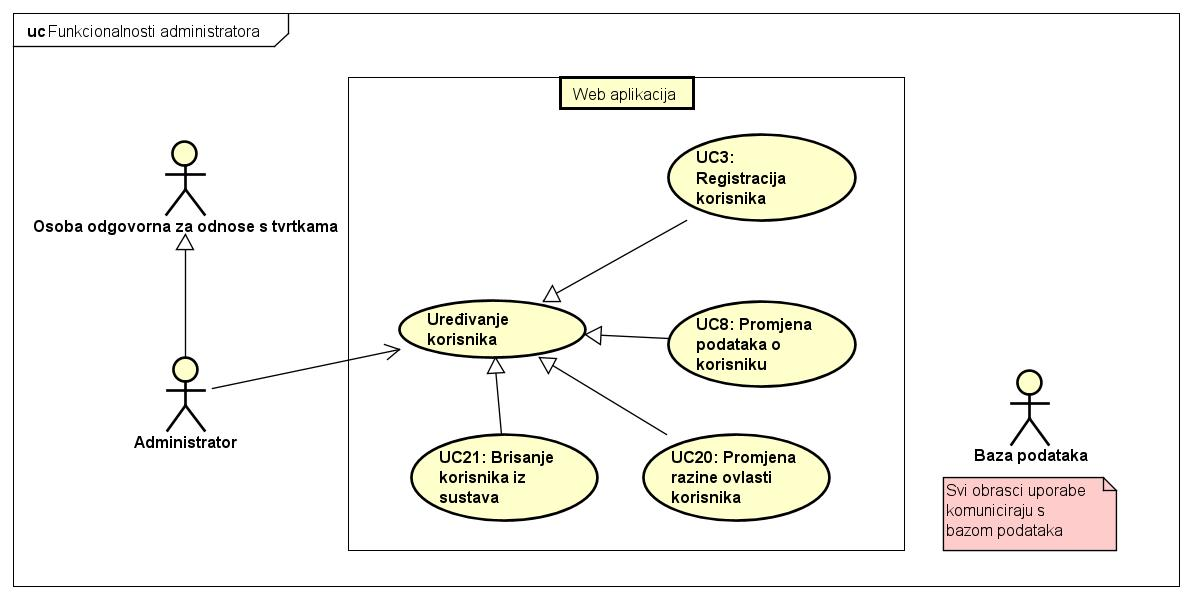
\includegraphics[width=1.25\textwidth]{./slike/UC dijagrami/UseCase administrator}
					\textit{Slika 3.5: Dijagram obrasca uporabe, funkcionalnosti administratora}

				\eject
				
			\subsection{Sekvencijski dijagrami}
				
				\textbf{\textit{dio 1. revizije}}\\
				
				\textit{Nacrtati sekvencijske dijagrame koji modeliraju najvažnije dijelove sustava (max. 4 dijagrama). Ukoliko postoji nedoumica oko odabira, razjasniti s asistentom. Uz svaki dijagram napisati detaljni opis dijagrama.}
				\eject
	
		\section{Ostali zahtjevi}
		
			\textbf{\textit{dio 1. revizije}}\\
		 
			 \textit{Nefunkcionalni zahtjevi i zahtjevi domene primjene dopunjuju funkcionalne zahtjeve. Oni opisuju \textbf{kako se sustav treba ponašati} i koja \textbf{ograničenja} treba poštivati (performanse, korisničko iskustvo, pouzdanost, standardi kvalitete, sigurnost...). Primjeri takvih zahtjeva u Vašem projektu mogu biti: podržani jezici korisničkog sučelja, vrijeme odziva, najveći mogući podržani broj korisnika, podržane web/mobilne platforme, razina zaštite (protokoli komunikacije, kriptiranje...)... Svaki takav zahtjev potrebno je navesti u jednoj ili dvije rečenice.}

			\begin{packed_item}

				\item \textit{Sustav treba omogućiti rad više korisnika u stvarnom vremenu}
				\item \textit{Korisničko sučelje i sustav moraju podržavati hrvatsku abecedu (dijakritičke
				znakove) pri unosu i prikazu tekstualnog sadržaja}
				\item \textit{Izvršavanje dijela programa u kojem se pristupa bazi podataka ne smije trajati
				duže od nekoliko sekundi}
				\item \textit{Sustav treba biti implementiran kao web aplikacija koristeći
				objektno- orijentirane jezike}
				\item \textit{Neispravno korištenje korisničkog sučelja ne smije narušiti funkcionalnost i
				rad sustava}
				\item \textit{Sustav treba biti jednostavan za korištenje, korisnici se moraju znati koristiti
				sučeljem bez opširnih uputa}
				\item \textit{Veza s bazom podataka mora biti kvalitetno zaštičena, brza i otporna na
				vanjske greske}
				\item \textit{Pristup sustavu mora biti omogućen iz javne mreže pomoču HTTPS}
				\item \textit{Prikazivanje stranice korisniku ne smije trajati dulje od desetak sekundi,
				bez obzira na količinu podataka koju prikazuje}

			\end{packed_item}
			 
	